
\section{Presto: Edge-based Load Balancing for Fast Datacenter Networks}
\label{presto}

\subsection{Introduction}
Presto is
a new load balancing scheme for data center networks. 
It utilizes the software edge (virtual switch in the hypervisor) and 
TCP offloading features (TCP Segmentation Offload and Generic Receive Offload) 
to achieve near-perfect traffic load balancing on symmetric 
networks (e.g., 2-tier Clos) with very little CPU overhead.
This work makes the following contributions:
\begin{enumerate}

\item We design and implement a system, called Presto, that near-optimally load balances
links in the network. We show that such a system can be built with no changes to the transport
layer or network hardware, and scales to 10+ Gbps networking speeds.
%Presto
%improves throughput, latency and fairness in the network and reduces flow completion time tail latencies
%for mice flows.
%\item We show that such a system can be built with no changes to the transport
%layer or within network hardware. Unlike previous approaches with similar design goals~\cite{drb}, we
%ensure our approach scales to network speeds higher than 1 Gbps.
Our approach makes judicious use of middleware
already implemented in most hypervisors today: Open vSwitch and the TCP receive offload engine in the OS
(Generic Receive Offload, GRO, in the Linux kernel).
\footnote{Also known as Receive Segment Coalescing (RSC)~\cite{ms-rsc}, 
or in hardware, Large Receive Offload (LRO)~\cite{grossman2005large}}

\item We uncover the importance of GRO on performance when packets are reordered.
At network speeds of 10+ Gbps, current GRO algorithms are unable to sustain line rate under
severe reordering due to extreme computational overhead, and hence
per-packet load-balancing approaches~\cite{cao2013drb,packetspray} need to be reconsidered. We
improve GRO to prevent reordering while ensuring computational overhead is limited.
%Our scheme can distinguish loss from reordering and adapt to prevailing network conditions.
%These techniques are criticial to ensure we minimize the time waiting for lost packets, while
%being robust against exposing reordering to higher network layers.
We argue
GRO is the most natural place to handle reordering because it can mask
reordering in a light-weight manner while simultaneously limiting CPU overhead by having a direct impact
on the segment sizes pushed up the networking stack.
%Need to sell this more: this is the only place we should really do it because it has
%direct impact on packet sizes, and thus CPU overhead. We also need to talk about mechanisms
%we create to distinguish loss from reordering.

\item Presto achieves near-optimal load balancing in a proactive manner. For that, it leverages symmetry in
the network topology to ensure that all paths between a pair of hosts are equally congested.
However, asymmetries can arise due to failures. We demonstrate Presto can recover from network failures and adapt to asymmetric
network topologies using a combination of fast failover and weighted multipathing at the network edge.

\item Finally, we evaluate Presto on a real 10 Gbps testbed. Our experiments show Presto
outperforms existing load balancing schemes (including flowlet switching, ECMP, MPTCP) and
is able to track the performance of a single, non-blocking switch (an optimal case) within a few percentage points
over a variety of workloads, including trace-driven. Presto improves throughput, latency and fairness in the network and
also reduces the flow completion time tail for mice flows.

\end{enumerate}


\subsection{Design Decisions and Challenges}
\label{sec:presto-background}

In Presto, we make several design choices to 
build a highly robust and scalable system that provides near optimal load 
balancing without requiring changes to the transport layer or switch hardware. We 
now discuss our design decisions.


\subsubsection{Design Decisions}

\tightparagraph{Load Balancing in the Soft Edge} A key design decision in Presto 
is to implement the functionality in the soft edge (\ie, the vSwitch and hypervisor) of 
the network. 
The vSwitch occupies a unique position in the networking stack 
in that it can easily modify packets without requiring any changes to customer VMs or transport layers.
Functionality built into the vSwitch can be made aware of the underlying hardware offload
features presented by the NIC and OS, meaning it can be fast.
Furthermore, an open, software-based approach prevents extra hardware cost and vendor 
lock-in, and allows for simplified network management. 
These criteria are important for providers today~\cite{amazon-peek}.
Thanks to projects like Open vSwitch, 
soft-switching platforms are now fast, mature, open source, adopted widely, remotely 
configurable, SDN-enabled, and feature-rich~\cite{pfaff2009extending,
koponen2014network}. Presto is built on these 
platforms.

\tightparagraph{Reactive vs Proactive Load Balancing} The second major design decision in 
Presto is to use a proactive approach to congestion management. Bursty 
behavior in datacenter workloads can create transient congestion issues that must be reacted to 
before switch buffers overflow to prevent loss (timescales range from hundreds of microseconds 
to ~4 ms~\cite{rasley2014planck}). This requirement renders most of the centralized reactive schemes ineffective
as they are often too slow to react to any but the largest network events,~\eg{}, link failures. 
Furthermore, centralized schemes can hurt performance when rerouting
flows using stale information.
Distributed reactive schemes like MPTCP~\cite{dc-mptcp} and 
CONGA~\cite{alizadeh2014conga} can respond to congestion at faster timescales, but have a high barrier to deployment.
Furthermore, distributed reactive schemes must take great care to avoid oscillations.
Presto takes a proactive, correct-by-design approach to congestion management. 
That is, if small, uniform portions of traffic are equally
balanced over a symmetric network topology, then we don't need to 
be reactive to congestion.
Presto is only reactive to network events such as link failures. Fortunately, 
the higher timescales of the reactive feedback loops are sufficient in these scenarios. 

\tightparagraph{Load Balancing Granularity} ECMP has been shown to be 
ineffective at load balancing the network, and thus many schemes advocate 
load balancing at a finer granularity than a 
flow~\cite{cao2013drb,alizadeh2014conga,juniper-vcf,packetspray}. 
A key factor impacting the choice of granularity is operating at high speed. 
Operating at 10+ Gbps incurs great computational overhead, and therefore host-based load balancing schemes
must be fast, light-weight and take advantage of optimizations provided in the networking stack.
For example, per-packet load balancing techniques~\cite{cao2013drb} cannot be
employed at the network edge because TSO does not work on a per-packet
basis. TSO, commonly supported in OSes and NICs, allows for large TCP segments (typically 64 KB in size)
to be passed down the networking stack to the NIC. The NIC breaks the segments into MTU-sized packets and copies and computes
header data, such as sequence numbers and checksums. When TSO is disabled, a host incurs 100\% CPU utilization and can only achieve
around 5.5 Gbps~\cite{bullettrains}. Therefore, per-packet schemes are unlikely to scale to fast networks without hardware support.
Limiting overhead by increasing the MTU is difficult because
VMs, switches, and routers must all be configured appropriately, and traffic
leaving the datacenter must use normal 1500 byte packets. 
Furthermore, per-packet schemes~\cite{cao2013drb,packetspray} are likely to
introduce significant reordering into the network.

\begin{figure}[t]
        \centering
  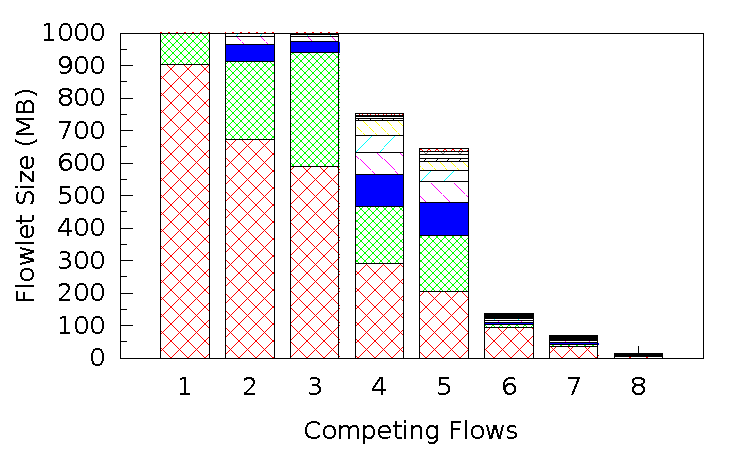
\includegraphics[width=0.55\textwidth]{./figures/presto/flowlets/histo.pdf}
        \caption{Stacked histogram of flowlet sizes (in MB) for a 1 GB {\tt scp} file transfer. We vary the number of {\tt nuttcp} background flows and
                denote them as {\em Competing Flows}. The size of each flowlet is shown within each bar, and flowlets
                are created whenever there is a 500 $\mu$s delay between segments. The top 10 flowlet sizes are shown here.
                We also analyzed the results of a 1 GB {\tt nuttcp}, {\tt ftp}, and a simple custom client/server transfer and found them
                to be similar. }
        \label{micro_flowlet_size}
\end{figure}


Another possibility is to load balance on flowlets~\cite{alizadeh2014conga,juniper-vcf}.  
A flow is comprised of a series of bursts, and a flowlet is created when
the inter-arrival time between two packets in a flow exceeds a threshold inactivity timer.  
In practice, inactivity timer values are between 100-500 $\mu$s~\cite{alizadeh2014conga}. 
These values intend to strike a good balance between load balancing on a sub-flow level 
and acting as a buffer to limit reordering between flowlets.
Flowlets are derived from traffic patterns at the sender, and in practice this
means the distribution of flowlet sizes is not uniform. To analyze flowlet sizes, a simple experiment is shown in Figure~\ref{micro_flowlet_size}. 
We connect a sender and a receiver to a single switch and start an {\tt scp} transfer designed to 
emulate an elephant flow. Meanwhile, other senders are hooked up to the same switch and
send to the same receiver. We vary the number of these competing flows and show a stacked histogram of 
the top 10 flowlet sizes for a 1 GB {\tt scp} transfer with a 500 $\mu$s inactivity timer. 
The graph shows flowlet sizes can be quite large, with more than half the transfer being attributed
to a single flowlet for up to 3 competing flows. Using a smaller inactivity timer, such 100$\mu$s, helps (90\% of flowlet sizes are 114KB or less), but
does not prevent a long tail: 0.1\% of flowlets are larger than 1 MB, with the largest ranging from 2.1-20.5 MB.
Collisions on large flowlet sizes can lead to congestion.
The second problem with flowlets is that small inactivity thresholds, such as 100 $\mu$s, can lead to significant reordering.
Not only does this impact TCP performance (profiled in \secref{sec:presto-eval}), 
but it also needlessly 
breaks small flows into several flowlets. With only one flow in the network, we found a 50 KB
mice flow was broken into 4-5 flowlets on average. Small flows typically do not need to be
load balanced on a sub-flow level and need not be exposed to reordering.


The shortcomings of the previous approaches lead us to reconsider on what granularity
load balancing should occur. 
Ideally, sub-flow load balancing should be done on near uniform sizes.
Also, the unit of load balancing should be small to
allow for fine-grained load balancing, but not so small as to break small flows into 
many pieces or as to be a significant computational burden. As a result, we
propose load balancing on 64 KB units of data we call {\em flowcells}. Flowcells
have a number of advantages. First, the maximum segment size supported by TSO
is 64 KB, so flowcells provide a natural interface to high speed optimizations provided
by the NIC and OS and can scale to fast networking speeds. Second, an overwhelming fraction of mice flows are less than 64 KB in size
 and thus do not have to worry about reordering~\cite{benson10,vl2,kandula2009nature}.
Last, since most bytes in datacenter networks originate from elephant flows~\cite{kandula2009nature,benson10,alizadeh2011dctcp},
this ensures that a significant portion of datacenter traffic is routed on uniform
sizes. While promising, this approach must combat reordering to be effective. 
Essentially we make a trade-off: we provide line rate load balancing in the most effective
manner as to avoid congestion and then handle reordering head-on at the receiver.

\tightparagraph{End-to-End vs Per-Hop Multipathing}
The last design consideration is whether multipathing should be done on a local, per-hop level (\eg{}, ECMP), or
on a global, end-to-end level. In Presto, we choose the latter: pre-configured end-to-end paths
are allocated in the network and path selection (and thus multipathing) is realized by having the network edge
place flowcells onto these paths. 
Presto can be used to load-balance in an ECMP style per-hop manner but the choice of end-to-end 
multipathing provides additional benefits due to greater control on how flowcells are mapped to
paths. Per-hop multipathing can be inefficient
under asymmetric topologies~\cite{zhou2014wcmp}, and load-balancing on a global end-to-end level can allow
for weighted scheduling at vSwitch to rebalance traffic. This is especially important when failure occurs.
The second benefit is that flowcells can be assigned over multiple paths very evenly
by iterating over paths in a round-robin, rather than randomized, fashion. 

\subsubsection{Reordering Challenges}
Due to the impact of fine-grained, flowcell-based load balancing, Presto must account for reordering. Here, we 
highlight reordering challenges. The next section shows how Presto deals with these concerns.

\tightparagraph{Reordering's Impact on TCP} The impact of reordering on TCP is well-studied~\cite{leung2007overview,paxson1997end}. 
Duplicate acknowledgments caused by reordering
can cause TCP to move to a more conservative sender state and reduce the sender's congestion window.
Relying on parameter tuning, such as adjusting the DUP-ACK threshold, is not ideal because 
increasing the DUP-ACK threshold increases the time to recover from real loss. Other TCP settings
such as Forward Acknowledgement (FACK) assume un-acked bytes in the SACK are lost and degrade
performance under reordering. 
A scheme that introduces reordering should not rely on careful configuration of TCP parameters
because (i) it is hard to find a single set of parameters that work effectively over multiple 
scenarios and (ii) datacenter tenants should not be forced to constantly tune their networking stacks.
Finally, many reordering-robust variants of TCP have been proposed~\cite{rr-tcp,blanton2002making,tcp-pr}, but
as we will show, GRO becomes ineffective under reordering. Therefore, reordering should
be handled below the transport layer.

\tightparagraph{Computational Bottleneck of Reordering}
Akin to TSO, Generic Receive Offload (GRO) mitigates the computational burden of receiving
1500 byte packets at 10 Gbps. GRO is implemented in the kernel of the hypervisor
and its handler is called directly by the NIC driver. It is responsible
for aggregating packets into larger segments that are pushed up to OVS and the TCP/IP stack.
Because modern CPUs use aggressive prefetching, the cost of receiving
TCP data is now dominated by per-packet, rather than per-byte, operations.
As shown by Menon~\cite{optimize-tcp-receive},  the majority of this overhead comes from
buffer management and other routines not related to protocol processing, and therefore 
significant computational overhead can be avoided by aggregating "raw" packets from
the NIC into a single {\tt sk\_buff}.\footnote{Refer to~\cite{optimize-tcp-receive} for detailed study and explanation}
Essentially, spending a few cycles to aggregate packets within GRO creates less segments for
TCP and prevents having to use substantially more cycles at higher layers in the networking stack.

To better understand the problems reordering causes, a brief description of  
the TCP receive chain in Linux follows. First, interrupt coalescing
essentially allows the NIC to create an interrupt for a batch of packets~\cite{mogul1997eliminating,understanding-linux-network},
which prompts the driver to poll the packets into an aggregation queue. Next, the driver
invokes the GRO handler, located in the kernel, which
{\em merges} the packets into larger segments. The merging continues,
possibly across many polling events, until a segment
reaches a threshold size, a certain age, or cannot be combined with the incoming packet. Then, the
combined, larger segment is {\em pushed up} to the rest of the TCP/IP networking stack. The GRO process is
done on a per-flow level. With GRO disabled, throughput drops to around
5.7-7.1 Gbps and CPU utilization spikes to 100\% (\secref{sec:presto-eval} and~\cite{bullettrains}). 
Receive offload algorithms, whether in hardware 
(LRO)~\cite{grossman2005large} or in software (GRO), are usually
{\em stateless} to make them fast: no state is kept beyond the segment being merged.


\begin{figure}[t]
        \centering
  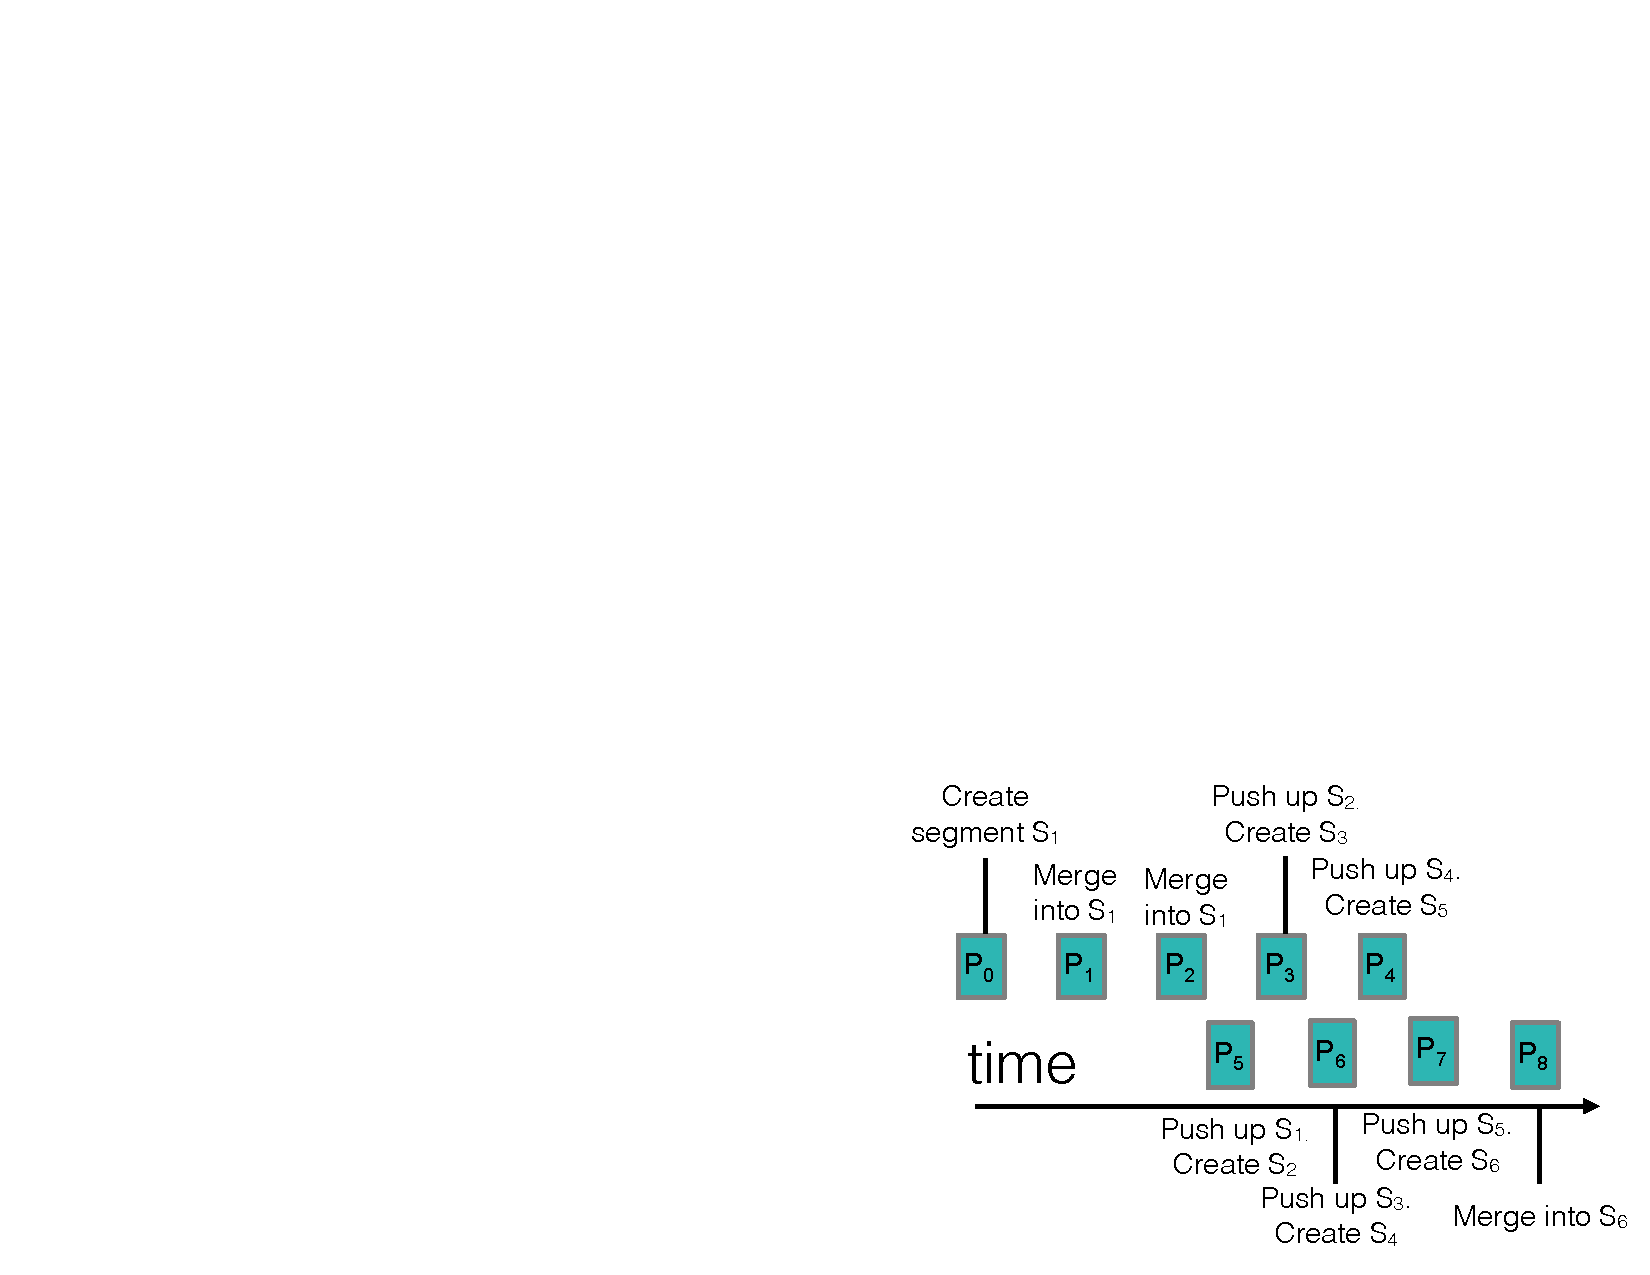
\includegraphics[width=0.55\textwidth]{./figures/presto/gro-design/gro-break.pdf}
        \caption{GRO pushes up small segments ($S_i$) during reordering.}
        \label{gro-break}
\end{figure}


We now uncover how GRO breaks down in the face of reordering. Figure~\ref{gro-break} shows the impact of reordering on GRO.  Reordering does not allow the segment to grow: each reordered packet cannot be merged with the existing segment, and thus the previously created segment must be pushed up. With extreme reordering, GRO is effectively disabled because small MTU-sized segments are constantly pushed up. This causes (i) severe computational overhead and (ii) TCP to be exposed to significant amounts of reordering. We term this the {\em small segment flooding} problem.

Determining where to combat the reordering problem has not previously taken the small segment flooding problem into account.  Using a reordering buffer to deal with reordered packets is a common solution (\eg{}, TCP does this, other works re-sort in a shim layer below TCP~\cite{cao2013drb}), but a buffer implemented above GRO cannot prevent small segment flooding.  Implementing a buffer below GRO means that the NIC must be changed, which is (i) expensive and cumbersome to update and (ii) unlikely to help combat reordering over multiple interrupts.

In our system, the buffer is implemented in the GRO layer itself.  We argue this is a natural location because GRO can
directly control segment sizes while simultaneously limiting the impact of reordering. 
Furthermore, GRO can still be applied on packets pushed up from LRO, which means hardware doesn't have to be modified
or made complex.
Implementing a better GRO has multiple challenges. The algorithm should be fast and light-weight to scale to fast networking speeds. Furthermore, an ideal scheme should be able to distinguish loss from reordering.  When a gap in sequence numbers is detected (\eg{}, when $P_5$ is received after $P_2$ in Figure~\ref{gro-break}), it is not obvious if this gap is caused from loss or reordering.  If the gap is due to reordering, GRO should not push segments up in order to try to wait to receive the missing gap and merge the missing packets into a preestablished segment.  If the gap is due to loss, however, then GRO should immediately push up the segments to allow TCP to react to the loss as fast as possible. Ideally, an updated GRO algorithm should ensure TCP does not perform any worse than a scheme with no reordering. Finally, the scheme should adapt to prevailing network conditions, traffic patterns and application demands.



\subsection{Design}
\label{sec:presto-design}

This section presents the design of Presto by detailing
the sender, the receiver, and how the network
adapts in the case of failures and asymmetry.

\begin{figure}[!t]
        \centering
  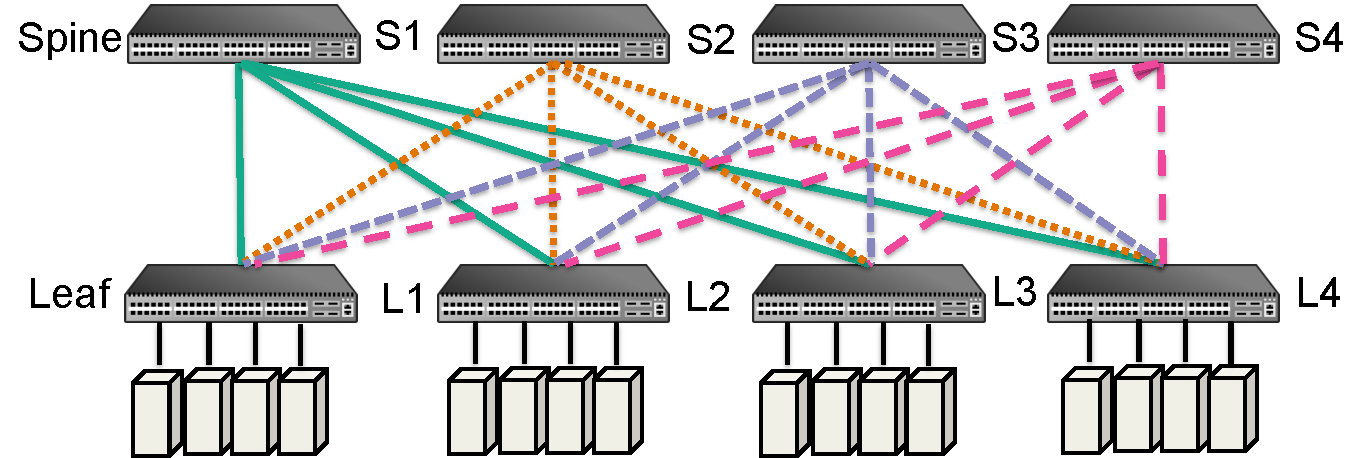
\includegraphics[width=0.55\textwidth,height=0.17\textwidth]{./figures/presto/macro/macro_evaluation_topology_refined.pdf}
        \caption{Our testbed: 2-tier Clos network with 16 hosts.}
        \label{macro_evaluation_topology}
\end{figure}

\subsubsection{Sender}


\tightparagraph{Global Load Balancing at the Network Edge}
In Presto, a centralized controller is employed to collect the
network topology and disseminate corresponding load balancing information to the edge vSwitches. 
The goal of this design is to ensure the vSwitches, as a whole, can load balance the network
in an even fashion, but without requiring an individual vSwitch to have detailed information
about the network topology, updated traffic matrices or strict coordination amongst senders.
 At a high level, the controller partitions
the network into a set of multiple spanning trees. Then, the controller
assigns each vSwitch a unique forwarding label in each spanning tree.
By having the vSwitches partition traffic over these spanning trees in a fine-grained
manner, the network can load balance traffic in a near-optimal fashion.

The process of creating spanning trees is made simple by employing multi-stage Clos
networks commonly found in datacenters. For example, in a 2-tier Clos network
with $\nu$ spine switches, the controller can easily allocate $\nu$ disjoint spanning
trees by having each spanning tree route through a unique spine switch. Figure~\ref{macro_evaluation_topology}
shows an example with four spine switches and four corresponding disjoint spanning trees.
When there are $\gamma$ links between each spine and leaf switch in a 2-tier Clos network,
the controller can allocate $\gamma$ spanning trees per spine switch.
Note that 2-tier Clos networks are scalable because they easily support a large number
of hosts with only a few high density spine switches~\cite{alizadeh2014conga}.
In general, the controller ensures links in the network are equally covered
by the allocated spanning trees.
Once the spanning trees are created, the controller assigns a unique forwarding label
for each vSwitch in every spanning tree and installs them into the network.
Forwarding labels can be implemented in a variety of ways using
technologies commonly deployed to forward on labels,
such as MPLS~\cite{casado2012fabric}, VXLAN~\cite{alizadeh2014conga,koponen2014network}, 
or IP encapsulation~\cite{cao2013drb}. 
In Presto,
label switching is implemented with shadow MACs~\cite{shadow-mac}. 
Shadow MACs implement label-switching for commodity Ethernet by using the 
destination MAC address as an opaque forwarding label that can easily be 
installed in L2 tables. 
Each vSwitch is assigned one shadow MAC per spanning tree.
Note Shadow MACs are extremely scalable on
existing chipsets because they utilize the large L2 forwarding table. For example,
Trident II-based switches~\cite{bcm-smart-table} have 288k L2 table entries and 
thus 8-way multipathing (\ie{}, each vSwitch has 8 disjoint spanning trees)
can scale up to 36,000 physical servers.


\tightparagraph{Load Balancing at the Sender}
After the controller installs the shadow MAC forwarding rules into the network, it creates a mapping
from each physical destination MAC address to a list of corresponding shadow MAC addresses. These mappings
provide a way to send traffic to a specific destination over different spanning trees. 
The mappings are pushed from the controller to each vSwitch in the network, either on-demand or preemptively.
In Presto, the vSwitch on the sender monitors outgoing traffic (\ie{}, maintains a per-flow counter in the datapath) 
and rewrites the destination MAC
address with one of the corresponding shadow MAC addresses.
The vSwitch assigns the same shadow MAC address to all consecutive segments until the 64 KB limit is reached.
In order to load balance the network effectively, the vSwitch 
iterates through destination shadow MAC addresses in a round-robin fashion. 
This allows the edge vSwitch to load balance over the network in a very fine-grained fashion.

Sending each 64 KB worth of flowcells over a different path in the network can cause reordering and must
be carefully addressed.
To assist with reordering at the receiver (Presto's mechanisms for combatting reordering are detailed in the next section), 
the sender also includes a sequentially increasing {\em flowcell ID} into each segment.
For example, 
in our setup the controller installs forwarding rules solely on the destination MAC address.
ARP is handled in a centralized manner, so
the source MAC address can be used to hold the flowcell ID. Other options are possible, 
\eg{}, some schemes include load balancing metadata in the reserved bits of the 
VXLAN header~\cite{presto-nvo3}.\footnote{In our
implementation, TCP options hold the flowcell ID for simplicity and ease of debugging.}
Note that since the flowcell ID and the shadow MAC address are modified before a segment is handed to the NIC,
the TSO algorithm in the NIC replicates these values to all derived MTU-sized packets.

\begin{algorithm}[t]
\caption{Pseudo-code of Presto GRO {\tt flush} function}
\label{alg:gro}
\begin{algorithmic}[1]
%\REQUIRE $n \geq 0 \vee x \neq 0$
%\ENSURE $y = x^n$
\FOR{each flow f}
\FOR{$S \in f.{\tt segment\_list}$}
%\STATE f = getFlow(S)
\IF{f.lastFlowcell == getFlowcell(S)}
\STATE f.expSeq $\leftarrow$ max(f.expSeq, S.endSeq)
\STATE pushUp(S)
\ELSIF{getFlowcell(S) $>$ f.lastFlowcell}
\IF{f.expSeq == S.startSeq}
\STATE f.lastFlowcell $\leftarrow$ getFlowcell(S)
\STATE f.expSeq $\leftarrow$ S.endSeq
\STATE pushUp(S)
\ELSIF{timeout(S)}
\STATE f.lastFlowcell $\leftarrow$ getFlowcell(S)
\STATE f.expSeq $\leftarrow$ S.endSeq
\STATE pushUp(S)
\ENDIF
\ELSE
\STATE pushUp(S)
\ENDIF
\ENDFOR
\ENDFOR
\end{algorithmic}
\end{algorithm}

\subsubsection{Receiver}
The main challenge at the receiver is dealing with reordering that can occur when different flowcells
are sent over different paths. The high level goal of our receiver implementation is
to mitigate the effects of the small segment flooding problem by (i) not so aggressively pushing
up segments if they cannot be merged with an incoming packet and (ii) ensuring that segments
pushed up are delivered in order.

\tightparagraph{Mitigating Small Segment Flooding} Let's use Figure~\ref{gro-break} as a motivating example 
on how to combat the small segment flooding problem. Say a polling event has occurred, and the driver retrieves
9 packets from the NIC ($P_0$-$P_8$). The driver calls the GRO handler, which tries to merge consecutive packets
into larger segments. The first three packets ($P_0$-$P_2$) are merged into a segment, call it $S_1$ (note: in practice
$S_1$ already contains in order packets received before $P_0$).
When $P_5$ arrives, a new segment $S_2$, containing $P_5$, should be created. Instead of pushing up $S_1$ (as is done currently),
both segments should be kept.
Then, when $P_3$ is received, it can be merged into $S_1$. Similarly, $P_6$ can be merged into $S_2$. This process
can continue until $P_4$ is merged into $S_1$. At this point, the gap between the original out-of-order reception ($P_2$-$P_5$)
 has been filled, and $S_1$ can be pushed up and $S_2$ can continue to grow. This means the size of the segments being pushed up is increased,
and TCP is not exposed to reordering.

The current default GRO algorithm works as follows. An interrupt by the NIC causes the driver to poll
(multiple) packets from the NIC's ring buffer. The driver calls the GRO handler on the received batch
of packets. GRO keeps a simple doubly linked list, called {\tt gro\_list}, that contains 
segments, with a flow having at most one segment in the list. When packets for a flow are
received in-order, each packet can be merged into the flow's preexisting segment. When a packet
cannot be merged, such as with reordering, the corresponding segment is pushed up (ejected from the
linked list and pushed up the networking stack) and a new segment is created from the packet. 
This process is continued until all packets in the batch are serviced. At the end 
of the polling event, a {\tt flush} function is called that pushes up all segments in the
{\tt gro\_list}.

Our GRO algorithm makes the following high-level changes. First, multiple segments can be
kept per flow, and each flow contains a doubly linked list of its segments (called {\tt segment\_list}). 
To ensure the merging process is fast each linked list is kept in a hash table (keyed on flow).
When an incoming packet cannot be merged with any existing segment, the existing
segments are kept and a new segment is created from the packet.
New segments are added to the head of the linked list so that merging subsequent packets is typically $\mathcal{O}(1)$.
When the merging is completed over all packets in the batch, the {\tt flush} function is called. 
The {\tt flush} function decides whether to push segments up or to keep them. Segments may 
be kept so reordered packets still in flight have enough time to arrive and can then be placed in order
before being pushed up. 
Reordering can cause the linked lists to become slightly out-of-order, so
at the beginning of {\tt flush} an insertion sort is run to help easily decide if segments are in order.

The pseudo-code of our {\tt flush} function is presented in Algorithm~\ref{alg:gro}.
For each flow, our algorithm keeps track of the next expected in-order
sequence number ({\tt f.expSeq}) and the corresponding flowcell ID
of the most recently received in-order sequence number ({\tt f.lastFlowcell}).
The {\tt flush} function iterates over 
the sorted segments ($S$), from lowest sequence number to highest sequence number, in the {\tt segment\_list} (line 2).
The rest of the code is presented in the subsections that follow.


\tightparagraph{How to Differentiate Loss from Reordering?} 
In the case of no loss or reordering, our algorithm keeps pushing up segments and updating state. Lines 3-5
deal with segments from the same flowcell ID, so we just need to update {\tt f.expSeq} each time. Lines 
6-10 represent the case when the current flowcell ID is fully received and we start to receive the
next flowcell ID. The problem, however, is when there is 
a gap that appears between the sequence numbers of the segments. When a gap is encountered,
it isn't clear if it is caused from reordering or from loss. If the gap is due to reordering,
our algorithm should be conservative and try to wait to receive the packets that "fill in the gap" 
before pushing segments up to TCP. If the gap is due to loss, however, then we should push up the 
segments immediately so that TCP can react to the loss as quickly as possible.

To solve this problem, we leverage the fact that all packets carrying the same flowcell ID traverse the 
same path and should be in order.
This means incoming sequence numbers can be monitored to check for
gaps. A sequence number gap within the same flowcell ID is assumed to be a loss, and not reordering,
so those packets are pushed up immediately (lines 3-5).
Note that because a flowcell consists of many packets (a 64KB flowcell consists
of roughly 42 1500 byte packets), when there is a loss, it is likely that it occurs within flowcell boundaries. 
The corner case, when a gap occurs on the flowcell boundary, leads us to the next design question.

\tightparagraph{How to Handle Gaps at Flowcell Boundaries?}
When a gap is detected in sequence numbers at flowcell boundaries, it is not clear if the gap is due
to loss or reordering. Therefore, the segment should be held long enough to
handle reasonable amounts of reordering, but not so long that TCP cannot respond
to loss promptly. Previous approaches that deal with reordering typically employ a large static
timeout (10ms)~\cite{cao2013drb}. 
Setting the timeout artificially high can handle reordering, but hinders TCP when the gap is
due to loss. 
Setting a lower timeout is difficult because it depends on many dynamic factors such as delays between
segments at the sender, amount of network congestion in different paths, and traffic patterns (multiple flows 
received at the same NIC affect inter-arrival time). 
As a result, we devise an adaptive timeout scheme, which monitors recent reordering events and sets a dynamic timeout value accordingly.
Presto tracks cases when there is reordering, but no loss, on flowcell boundaries and keeps an exponentially-weighted
moving average ($EWMA$) over these times. Presto then applies a timeout of $\alpha * EWMA$ to a segment when a gap is 
detected on flowcell boundaries. 
Here $\alpha$ is an empirical parameter that allows for timeouts to grow. As a further optimization, if a segment
has timed out, but a packet has been merged into that segment in the last $\frac{1}{\beta} * EWMA$ time interval, then 
the segment is still held in hopes of preventing reordering. We find $\alpha$ and $\beta$
work over a wide range of parameters and set both of them to 2 in our experiments. A timeout firing is dealt with in lines 11-15.


\subsubsection{Failure Handling and Asymmetry}
When failures occur, Presto relies on the controller to update the forwarding
behavior of the affected vSwitches. The controller can simply prune the spanning
trees that are affected by the failure, or more generally enforce a weighted
scheduling algorithm over the spanning trees.
Weighting allows for Presto to evenly distribute traffic over an asymmetric topology.
Path weights can be implemented in a simple fashion by duplicating shadow MACs used in
the vSwitch's round robin scheduling algorithm.
For example, assume we have three paths in total ($p_1$, $p_2$ and $p_3$) and their updated weights are 0.25, 0.5 and 0.25 respectively.
Then the controller can send the sequence of $p_1$, $p_2$, $p_3$, $p_2$ to the vSwitch, which
can then schedule traffic over this sequence in a round robin fashion to realize the new path weights.
This way of approximating path weights in the face of network
asymmetry is similar to WCMP~\cite{zhou2014wcmp}, but instead of having to change switch firmware and use
scarce on-chip SRAM/TCAM entries, we can push the weighted load balancing entirely to the network edge.

As an added optimization, Presto can leverage any fast failover features that 
the network supports, such as BGP fast external failover, MPLS fast reroute, or OpenFlow failover groups. Fast failover detects port failure and can move corresponding traffic
to a predetermined backup port.
\footnote{Hardware failover latency ranges from several to 
tens of milliseconds}
This ensures traffic is moved away from the failure rapidly and the network
remains connected when redundant links are available.
Moving to backup links causes imbalance in the network,
so Presto relies on the controller learning of the network change, computing weighted multipath schedules, and
disseminating the schedules to the vSwitches. 


\subsection{Methodology}
\label{sec:presto-method}

\tightparagraph{Implementation}
We implemented Presto in Open vSwitch v2.1.2 and Linux kernel v3.11.0.
In OVS, we modified 5 files and $\sim$600 lines of code. For GRO, we modified 11 files and $\sim$900 lines of code.

\tightparagraph{Testbed} We conducted our experiments on a physical
testbed consisting of 16 IBM System x3620 M3 servers with 6-core Intel Xeon
2.53GHz CPUs, 60GB memory, and Mellanox ConnectX-2 EN 10GbE NICs. 
The servers were connected in a 2-tier Clos network topology with 10Gbps
IBM RackSwitch G8264 switches, as shown in Figure~\ref{macro_evaluation_topology}.

\tightparagraph{Experiment Settings}
We ran the default TCP implementation in the Linux kernel (TCP CUBIC)
and set {\tt tcp\_sack}, {\tt tcp\_fack}, {\tt tcp\_low\_latency} to 1 unless otherwise noted. 
Further, we tuned the host RSS and IRQ affinity settings and kept them the same in all experiments.

\tightparagraph{Workloads}
We evaluate Presto with a set of synthetic and realistic workloads. 
Similar to previous works~\cite{al2010hedera,rasley2014planck}, 
our synthetic workloads include:

{\em Shuffle}: Each server in the testbed sends 1GB data to every other server in the testbed in random order. 
Each host sends two flows at a time. %The shuffle is finished if all the servers have finished their jobs. 
This workload emulates the shuffle behavior of MapReduce/Hadoop workloads.

{\em Stride(8)}: We index the servers in the testbed from left to right. In stride(8) workload, server[i] sends to server[(i+8) mod 16].

{\em Random}: Each server sends to a random destination 
 not in the same pod as itself. Multiple senders can send to the same receiver.

{\em Random Bijection}: Each server sends to a random destination not in the same pod as itself. 
Different from random, each server only receives data from one sender.
 
Finally, we also evaluate Presto with trace-driven workloads from real datacenter traffic~\cite{kandula2009nature}.

\tightparagraph{Performance Evaluation}
We compare Presto to ECMP, MPTCP, and a 
single non-blocking switch used to represent an optimal scenario.
ECMP is implemented by enumerating all possible end-to-end paths and randomly selecting a path for each flow.
MPTCP uses ECMP to determine the paths of each of its sub-flows.
The MPTCP implementation is still under active development, and
we spent significant effort in finding the most stable configuration of MPTCP on our testbed. Ultimately, we found that Mellanox {\tt mlx\_en4} driver version
2.2, MPTCP version 0.88, subflow count set to 8, OLIA congestion control algorithm, and configured buffer sizes
as recommended by~\cite{dc-mptcp} gave us the best trade-offs in terms of throughput, latency, loss and stability.
Unfortunately, despite our efforts, we still occasionally witness some stability issues 
with MPTCP that we believe are due to implementation bugs.

We evaluate Presto on various performance metrics, including: 
throughput (measured by {\tt nuttcp}), 
round trip time (a single TCP packet, measured by {\tt sockperf}), 
mice flow completion time (time to send a 50 KB flow and receive an application-layer acknowledgement), packet loss (measured from switch counters), 
and fairness (Jain's fairness index over flow throughputs).  Mice flows are sent every 100 ms and elephant flows last 10 seconds. 
Each experiment is run for 10 seconds over 20 runs. Error bars on graphs denote
the highest and lowest value over all runs.


%\subsection{Microbenchmarks}
\label{sec:presto-micro}

We first evaluate the effectiveness of Presto over a series of microbenchmarks. Using 
canonical topologies, we investigate (i) Presto's effectiveness in preventing the small segment
flooding problem and reordering, (ii) Presto's CPU overhead, (iii) Presto's ability to scale
to multiple paths, (iv) Presto's ability to handle congestion, (v) comparison to flowlet
switching, and (vi) comparison to local, per-hop load balancing.

%%%%%micro test - scalability and congestion test topology
\begin{figure}[t]
        \centering
	\begin{subfigure}[b]{0.40\textwidth}
        	\centering
  		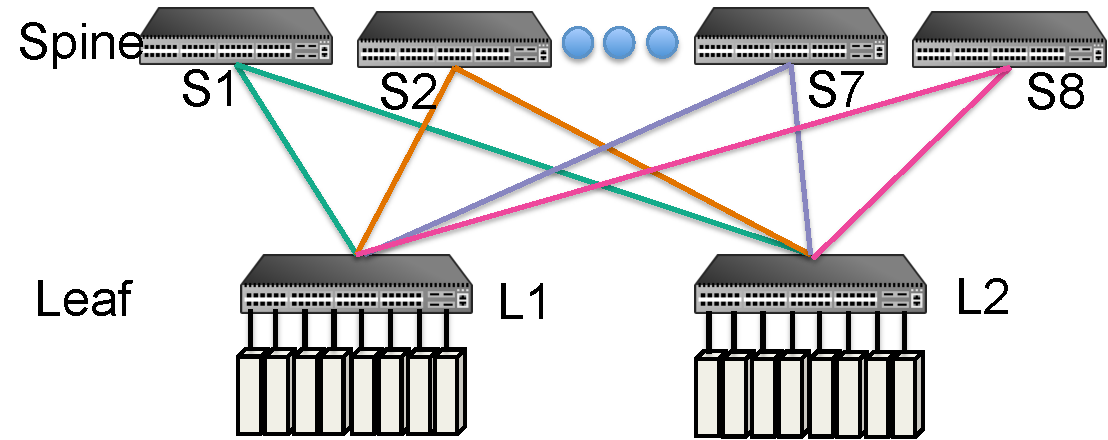
\includegraphics[width=\textwidth]{./figures/presto/micro_test_topology/micro_scalabilitytest_topology_refined.pdf}
        	\caption{}
		\label{micro_scalability_topology}
	\end{subfigure}
	\begin{subfigure}[b]{0.40\textwidth}
                \centering
		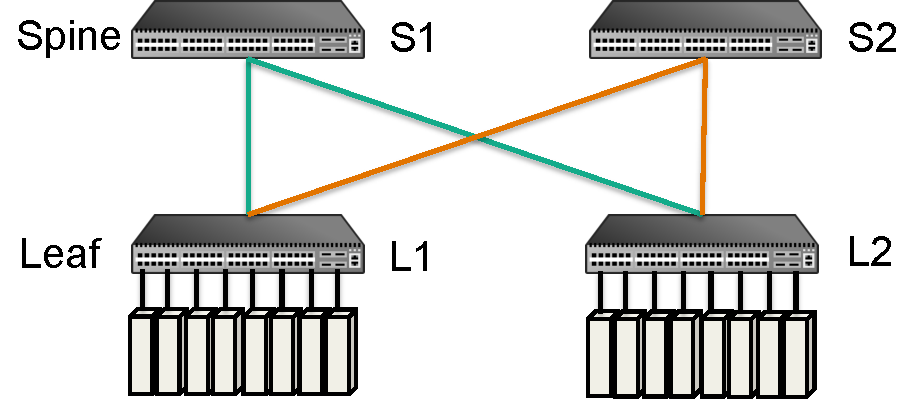
\includegraphics[width=\textwidth]{./figures/presto/micro_test_topology/micro_congestiontest_topology_refined.pdf}
        	\caption{}
		\label{micro_congestion_topology}
	\end{subfigure}
	\caption{(a) Scalability benchmark and (b) Oversubscription benchmark topology.}
	\label{micro_topology}
\end{figure}

%%%%%gro effectiveness shows
\begin{figure}[t]
	\centering
	\begin{subfigure}[b]{0.35\textwidth}
                \centering
  		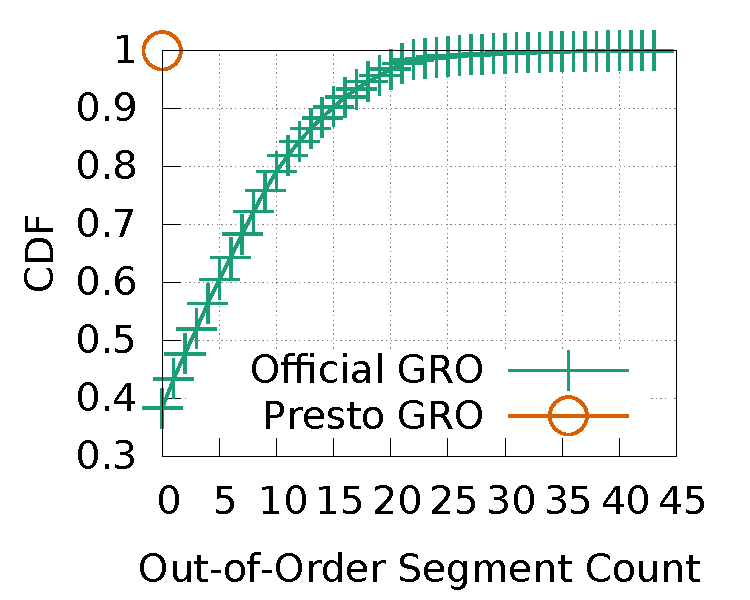
\includegraphics[width=\textwidth]{./figures/presto/gro_effectiveness/metric1_seg_cdf_compare.pdf}
		\caption{}
		\label{gro_effectiveness_on_reordering}
	\end{subfigure}
        \begin{subfigure}[b]{0.35\textwidth}
                \centering
		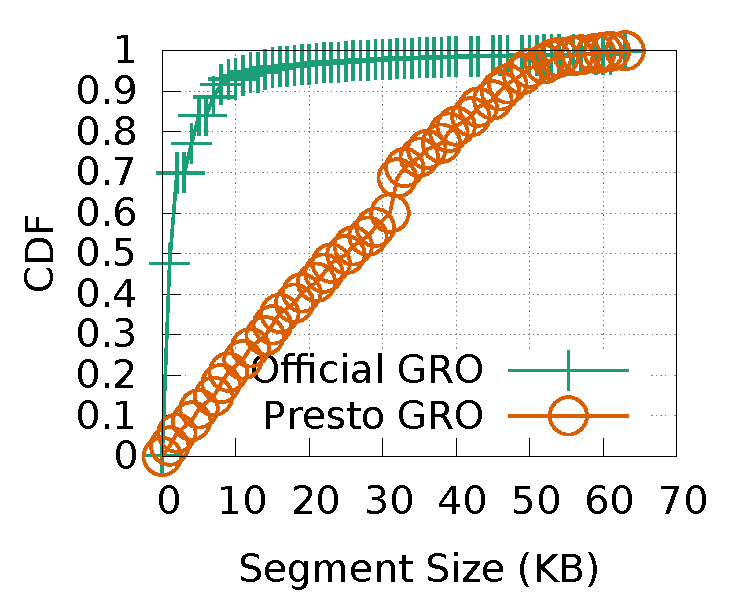
\includegraphics[width=\textwidth]{./figures/presto/gro_effectiveness/metric1_pktsize_cdf_compare.pdf}
        	\caption{}
		\label{gro_effectiveness_on_pktsize}
	\end{subfigure}
	\caption{(a) Illustration of the modified GRO's effectiveness on masking reordering. 
		(b) In case of massive packet reordering, official GRO cannot merge packets effectively such that lots of small
                packets are processed by TCP which poses great processing overhead for CPU.}
	\label{gro_effectiveness}
\end{figure}

\tightparagraph{Presto's GRO Combats Reordering}
To examine Presto's ability to handle packet reordering, we perform a simple experiment
on topology shown in Figure~\ref{micro_congestion_topology}.
Here two servers attached to leaf switch L1 
send traffic to their own receivers attached to leaf switch L2
by spreading 64KB flowcells over the two network paths. 
This setup can cause reordering for each flow, so 
we compare Presto's GRO to
an unmodified GRO, denoted "Official GRO". 
The amount of reordering exposed to TCP is presented in Figure~\ref{gro_effectiveness_on_reordering}.
To quantify packet reordering, we show a CDF of the {\em out-of-order segment count}:~\ie{},
the number of segments from other flowcells between the first packet and last packet of each flowcell. A value of zero
means there is no reordering and larger values mean more reordering. The figure shows Presto's GRO can completely mask reordering
while official GRO incurs significant reordering. As shown in Section~\ref{sec:presto-background}, reordering can
also cause smaller segments to be pushed up the networking stack, causing significant processing overhead.
Figure~\ref{gro_effectiveness_on_pktsize} shows the received TCP segment size distribution.  Presto's GRO
pushes up large segments, while the official GRO pushes up many small segments.
The average TCP throughputs in official GRO and Presto GRO are 4.6Gbps (with 86\% CPU utilization) and 
9.3Gbps (with 69\% CPU utilization), respectively. Despite the fact that official GRO only obtains 
about half the throughput of Presto's GRO, it still incurs more than 24\% higher CPU overhead. 
Therefore, an effective scheme must deal with both reordering and small segment overhead.

\begin{figure}[t]
        \centering
  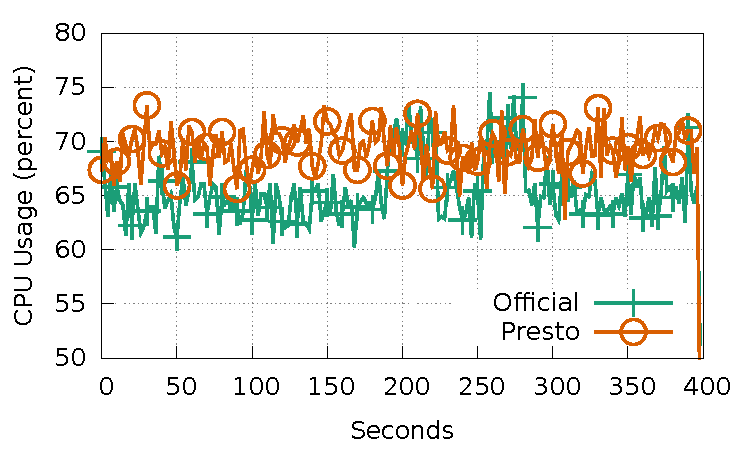
\includegraphics[width=0.55\textwidth]{./figures/presto/mornitor_cpu/macro_compare_cpu_usage.pdf}
        \caption{Presto incurs 6\% CPU overhead on average.}
        \label{micro_compare_cpu}
\end{figure}

\tightparagraph{Presto Imposes Limited CPU Overhead}
We investigate Presto's CPU usage by
running the stride workload on a 2-tier Clos network as shown in Figure~\ref{macro_evaluation_topology}. 
For comparison, official GRO is run with the stride workload using a non-blocking switch (so there
is no reordering). Note both official GRO and Presto GRO can achieve 9.3Gbps.  
The receiver CPU usage is sampled every 2 seconds over a 400 second interval, and
the time-series is shown in Figure~\ref{micro_compare_cpu}. 
On average, Presto GRO only increases CPU usage by 6\% compared with the official GRO. 
The minimal CPU overhead comes from Presto's careful design and implementation. 
At the sender, Presto needs just two {\tt memcpy} operations (1 for shadow MAC rewriting, 1 for flowcell ID encoding). 
At the receiver, Presto needs one {\tt memcpy} to rewrite the shadow MAC back to the real MAC and
also incurs slight overhead because multiple segments are now kept per flow. The overhead
of the latter is reduced because these segments are largely kept in reverse sorted order, which means {\tt merge}
on an incoming packet is usually $\mathcal{O}(1)$. The insertion sort is done at the beginning of each {\tt flush} event over a small
number of mostly in-order segments, which easily amortizes overhead because it is called infrequently compared to {\tt merge}.


\begin{figure}[t]
        \centering
  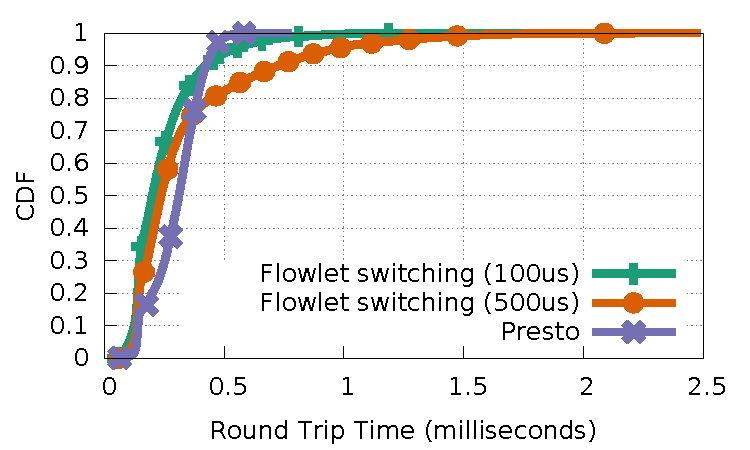
\includegraphics[width=0.55\textwidth]{./figures/presto/flowlets/flowlet_switching/flowlet_presto_compare_sockperf.pdf}
        \caption{Round trip time comparison of Flowlet switching~\cite{flowlet,alizadeh2014conga} and Presto in Stride workload. 
		The throughputs of Flowlet switching with 100 $\mu\text{s}$ gap, 500 $\mu\text{s}$ gap and Presto 
		are 4.3Gbps, 7.6Gbps and 9.3Gbps respectively. }
        \label{micro_flowlet_rtt_compare}
\end{figure}


\tightparagraph{Comparison to Flowlet Switching}
We implemented a flowlet load-balancing scheme in OVS that detects
inactivity gaps and then schedules flowlets over disjoint paths in a round robin fashion
(Presto does this over flowcells instead of flowlets).
The receiver for flowlets uses official GRO.
Presto is compared to 500 $\mu$s and 100 $\mu$s inactivity timers in
the stride workload on the 2-tier Clos network (Figure~\ref{macro_evaluation_topology}).
The throughput of the schemes are 9.3 Gbps (Presto), 7.6 Gbps (500 $\mu$s), and 4.3 Gbps (100 $\mu$s).
Analysis of the 100 $\mu$s
network traces show 13\%-29\% packets in the connection are reordered, which means 100 $\mu$s is not enough
time to allow packets to arrive in-order at the destination and thus throughput is severely impacted. Switching flowlets with 500 $\mu$s prevents
most reordering (only 0.03\%-0.5\% packets are reordered), but creates very large flowlets (see Figure~\ref{micro_flowlet_size}). This means
flowlets can still suffer from collisions, which can hurt throughput (note: while not shown here, 500 $\mu$s outperforms ECMP by over 40\%).
Figure~\ref{micro_flowlet_rtt_compare} shows the
latencies. Flowlet 100 $\mu$s has low throughput and hence lower latencies. However, since
its load balancing isn't perfect, it can still cause increased congestion in the tail. Flowlet 500 $\mu$s
also has larger tail latencies because of more pronounced flowlet collisions. As compared to the flowlet
schemes, Presto decreases 99.9$^{th}$ percentile latency by 2x-3.6x.



\subsection{Evaluation}
\label{sec:presto-eval}

In this section, we analyze the performance of Presto for (i) synthetic workloads, (ii)
trace-driven workloads, (iii) workloads containing north-south cross traffic, and (iv) failures.
All tests are run on the topology in Figure~\ref{macro_evaluation_topology}.
\begin{figure}[!t]
        \centering
  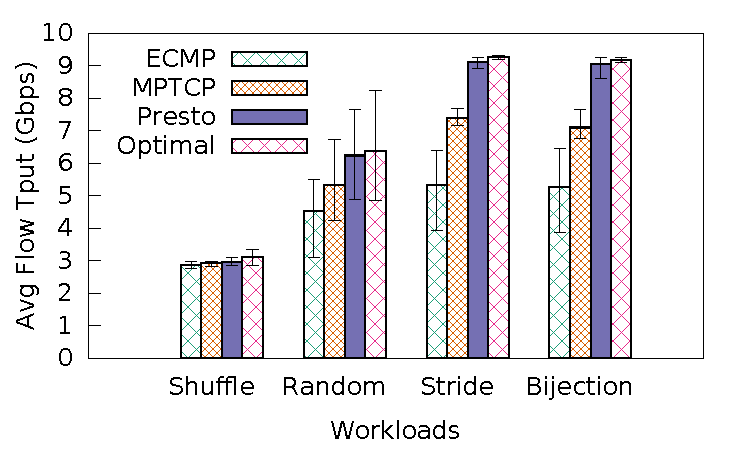
\includegraphics[width=0.55\textwidth]{./figures/presto/macro/stride/macro_compare_tput_witherrbar.pdf}
        \caption{Elephant flow's throughputs of ECMP, MPTCP, Presto and Optimal in Shuffle, Random, Stride and Random Bijection workloads.}
        \label{macro_evaluation_tput}
\end{figure}



\begin{figure*}[!t]
        \centering
	\begin{subfigure}[b]{0.3\textwidth}
                \centering
  		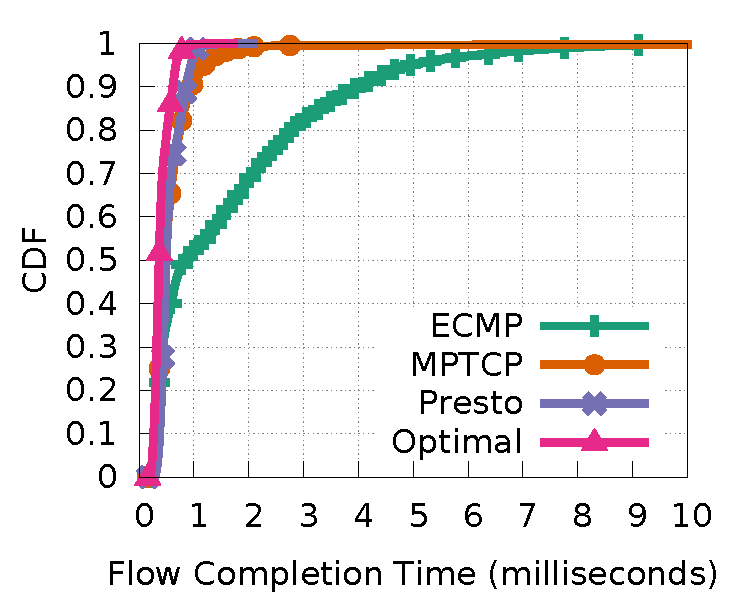
\includegraphics[width=\textwidth]{./figures/presto/macro/stride/macro_compare_fct_stride_mice.pdf}
        	\caption{Stride}
        	\label{macro_evaluation_fct_stride}
	\end{subfigure}
	\begin{subfigure}[b]{0.3\textwidth}
                \centering
		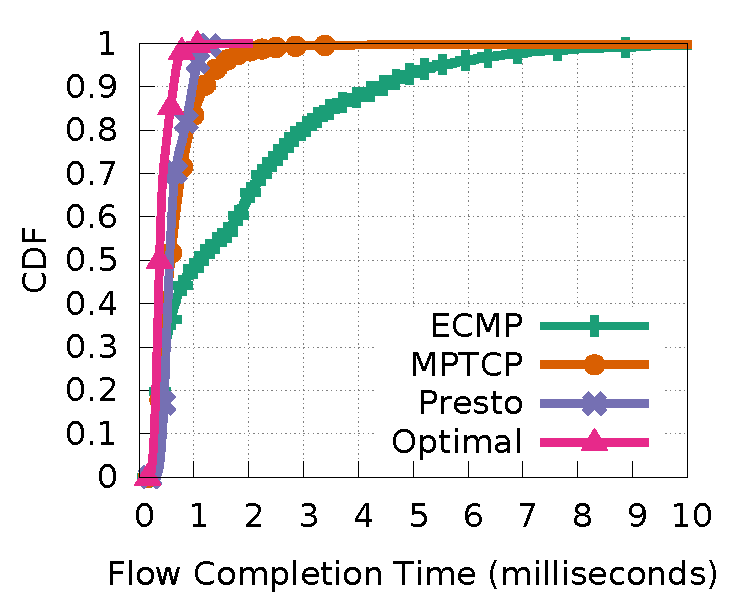
\includegraphics[width=\textwidth]{./figures/presto/macro/bijection/macro_compare_fct_bijection_mice.pdf}
        	\caption{Random Bijection}
        	\label{macro_evaluation_fct_bijection}
	\end{subfigure}
        %\begin{subfigure}[b]{0.225\textwidth}
        %        \centering
	%	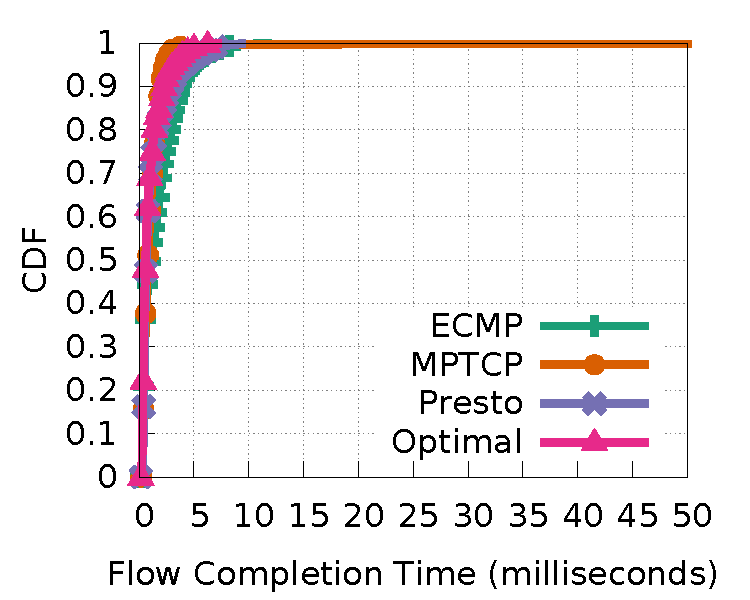
\includegraphics[width=\textwidth]{./figures/macro/random/macro_compare_fct_random_mice.pdf}
        %	\caption{Random}
        %	\label{macro_evaluation_fct_random}
	%\end{subfigure}
        \begin{subfigure}[b]{0.3\textwidth}
                \centering
		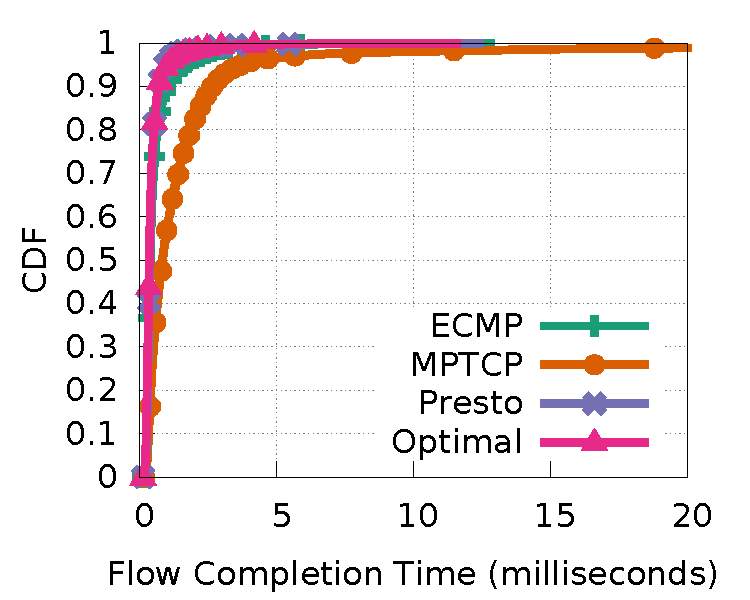
\includegraphics[width=\textwidth]{./figures/presto/macro/shuffle/macro_compare_fct_shuffle_mice.pdf}
        	\caption{Shuffle}
        	\label{macro_evaluation_fct_shuffle}
	\end{subfigure}
	\caption{Mice FCT of ECMP, MPTCP, Presto and Optimal in stride, random bijection, and shuffle workloads.}
	\label{macro_evaluation_fct}
\end{figure*}

\tightparagraph{Synthetic Workloads}
Figure~\ref{macro_evaluation_tput} 
shows the average throughputs of elephant flows in the shuffle, random, stride and random bijection workloads.
Presto's throughput is within 1-4\% of Optimal over all workloads.
For the shuffle workload, ECMP, MPTCP, Presto and Optimal show similar results 
because the throughput is mainly bottlenecked at the receiver. 
In the non-shuffle workloads, Presto improves upon ECMP by 38-72\% and improves
upon MPTCP by 17-28\%.

Figure~\ref{macro_evaluation_fct} shows the mice flow completion time (FCT) in
the workloads. 
The stride and random bijection workloads are non-blocking, and hence the latency of Presto
closely tracks Optimal: the 99.9$^{th}$ percentile FCT for Presto is within 350 $\mu$s for these workloads.
MPTCP and ECMP suffer from congestion, and therefore the tail FCT is much worse than Presto: ECMP's 99.9$^{th}$ percentile
FCT is over 7.5x worse ($\sim$11ms) and MPTCP experiences timeout (because of higher loss
rates and the fact that small sub-flow window sizes from small flows can increase the chances of timeout~\cite{dc-mptcp}).\footnote{We used the Linux default (200ms) and trimmed graphs for clarity}
The difference in the random and shuffle workloads is less pronounced (we omit random due to space constraints).
In these workloads elephant flows can collide on the last hop output port,
and therefore mice FCT is mainly determined by queuing latency. In shuffle, the 99.9$^{th}$ percentile FCT for ECMP, Presto and Optimal
are all within 10\% (MPTCP again experiences TCP timeout) and in random, the 99.9$^{th}$ percentile FCT of Presto is within 25\% of Optimal while ECMP's 
is 32\% worse than Presto.

%%% trace-driven workload, MSR, scaling factor =10
\begin{table}[!tb]
\begin{center}
\begin{tabular}{ |c|c|c|c| }
 \hline
 Percentile & ECMP & Optimal &Presto \\
 \hline
 50\%   & $1.0$ & $-12\%$ & $-9\%$   \\
 90\%   & $1.0$ & $-34\%$ & $-32\%$  \\
 99\%   & $1.0$ & $-63\%$  & $-56\%$ \\
 99.9\% & $1.0$ & $-61\%$ & $-60\%$  \\
 \hline

\end{tabular}
\caption{Mice ($<$100KB) FCT in trace-driven workload~\cite{kandula2009nature}. Negative numbers imply shorter FCT.}
        \label{macro_evaluation_MSR_trace_driven}
\end{center}
\end{table}

\tightparagraph{Trace-driven Workload}
We evaluate Presto using a trace-driven workload based on traffic patterns measured in~\cite{kandula2009nature}. 
Each server establishes a long-lived TCP connection 
with every other server in the testbed. 
Then each server continuously samples flow sizes and inter-arrival times and each time sends to a random receiver
that is not in the same rack.
We scale the flow size distribution by a factor of 10 to emulate a heavier workload. 
Mice flows are defined as flows that are less than 100 KB in size, and elephant flows are defined as flows
that are greater than 1 MB. The mice FCT, normalized to ECMP, 
is shown in Table~\ref{macro_evaluation_MSR_trace_driven}. 
Compared with ECMP, Presto has similar performance at the 50$^{th}$ percentile but reduces the 99$^{th}$ and 99.9$^{th}$ percentile FCT by 56\% and 60\%, respectively. 
Note MPTCP is omitted because its performance was quite unstable in workloads
featuring a large number of small flows.
The average throughput (not shown) for Presto tracks Optimal (within 2\%), and improves upon ECMP by over 10\%.


\begin{table}[!htb]
\begin{center}
\begin{tabular}{ |c|c|c|c|c| }
 \hline

 Percentile & ECMP & Optimal & Presto & MPTCP \\
 \hline
 50\%       & 1.0 & $-34$\%     & $-20$\%   & $-12$\% \\
 90\%       & 1.0 & $-83$\%     & $-79$\%   & $-73$\% \\
 99\%       & 1.0 & $-89$\%     & $-86$\%   & $-73$\% \\
 99.9\%     & 1.0 & $-91$\%      & $-87$\%   & TIMEOUT \\

 \hline
\end{tabular}
\caption{FCT comparison (normalized to ECMP) with ECMP load balanced north-south traffic.}
	\label{macro_evaluation_north_south_traffic}
\end{center}
\end{table}


\tightparagraph{Impact of North-South Cross Traffic}
Presto load balances on ``east-west'' traffic in the datacenter, \ie{}, traffic
originating and ending at servers in the datacenter. 
In a real datacenter environment "north-south" traffic (\ie{}, traffic with an endpoint outside the datacenter)
must also be considered. 
To study the impact of north-south traffic on Presto, we attach an additional server to 
each spine switch in our testbed to emulate remote users. 
The 16 servers establish a long-lived TCP connection with each remote user. 
Next, each server starts a flow to a random remote user every 1 millisecond. This emulates  
the behavior of using ECMP to load balance north-south traffic.
The flow sizes for north-south traffic are based on the distribution measurement in~\cite{he2013next}. 
The throughput to remote users is limited to 100Mbps to emulate the limitation of an Internet WAN. 
Along with the north-south flows, 
a stride workload is started to emulate the east-west traffic. 
The east-west mice FCT is shown in Table~\ref{macro_evaluation_north_south_traffic} (normalized to ECMP). 
ECMP, MPTCP, Presto, and Optimal's average throughput is 
5.7, 7.4, 8.2, and 8.9Gbps respectively. 
The experiment shows Presto can gracefully co-exist with north-south cross traffic
in the datacenter.


%%%failure handling experiments

\begin{figure}[t]
        \centering
  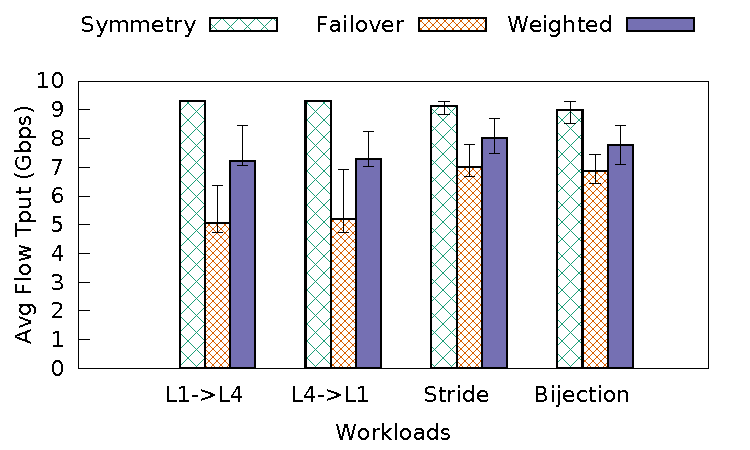
\includegraphics[width=0.55\textwidth]{./figures/presto/failure_handling/failover_compare_tput_witherrbar.pdf}
        \caption{Presto's throughput in symmetry, fast failover and weighted multipathing stages for different workloads.}
        \label{failover_compare_tput}
\end{figure}

\begin{figure}[t]
        \centering
  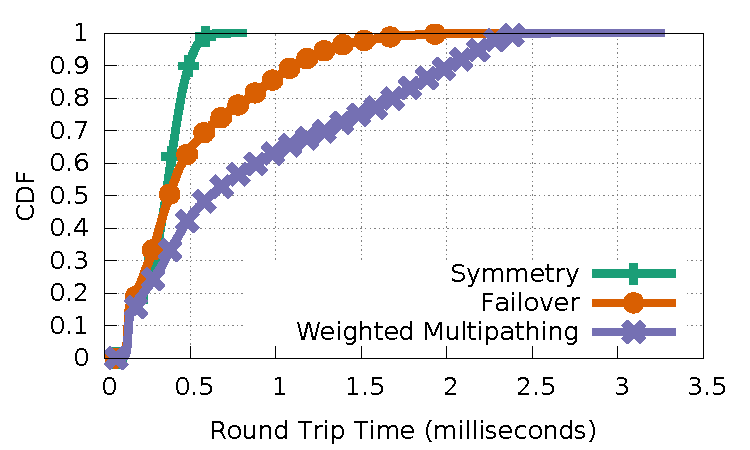
\includegraphics[width=0.55\textwidth]{./figures/presto/failure_handling/failover_compare_sockperf_bijection_mice.pdf}
        \caption{Presto's RTT in symmetry, fast failover and weighted multipathing stages in  random bijection workload.}
        \label{failover_compare_sockperf_bijection}
\end{figure}

\tightparagraph{Impact of Link Failure}
Finally, we study the impact of link failure.
Figure~\ref{failover_compare_tput} compares the throughputs of
Presto when %under different stages of loss recovery when 
the link between spine switch S1 and leaf switch L1 goes down.
Three stages are defined: symmetry (the link is up), failover (hardware fast-failover moves traffic from S1 to S2), and weighted (the controller
learns of the failure and prunes the tree with the bad link).
Despite the asymmetry in the topology, Presto still achieves reasonable average throughput at 
each stage.
Figure~\ref{failover_compare_sockperf_bijection} shows the round trip time of
each stage in a random bijection workload. 
Workload L1$\rightarrow$L4 is when each node connected to L1 sends to one node in L4 
(L4$\rightarrow$L1 is the opposite).
Due to the fact that the network is no longer non-blocking after the link failure,
failover and weighted multipathing stages have larger round trip time.

%\subsection{Conclusion}
\label{sec:presto-conclusion}
Presto is a near uniform sub-flow distributed load balancing scheme
that can near optimally load balance the network at fast networking speeds.
Our scheme makes a few simple changes to the hypervisor soft-edge (vSwitch and GRO)
and does not require any modifications to the transport layer or network hardware, making
the bar for deployment lower. 
Presto is explicitly designed to load balance the network at fine granularities
and deal with reordering without imposing too much overhead on hosts. Presto is flexible and can also
deal with failures and asymmetry. Finally, we show the performance of Presto can closely track
that of an optimal non-blocking switch, meaning elephant throughputs remain high while the tail
latencies of mice flow completion times do not grow due to congestion.

